\chapter{Introduction} \label{chap:intro}
\pagestyle{plain}
\setcounter{page}{1}

Informally, a \textit{distributed system} is a collection of independent 
computing entities (interchangeably called processes, actors, 
nodes, or participants) that communicate and coordinate their 
actions through message passing over a medium of communication 
(typically an \textbf{asynchronous network}), with the goal of solving a 
common problem. For example, a client-server application can be seen 
as a form of distributed system, where the shared objective is to provide 
services to an end user.

Distributed systems address a wide range of challenges which are 
difficult to solve without such an architecture, for example reliability
under failures safety in critical systems, and consistency of data.
% Being able to \textbf{scale} to handle large volumes of incoming requests 
% would be nearly impossible without distributed systems. Likewise, achieving 
% \textbf{fault-tolerant} and high-performance applications would be 
% extremely difficult without them. 
% For these reasons,
Distributed systems are 
widely adopted in domains such as \textit{cloud computing}, critical 
infrastructures, and telecommunication-oriented applications (i.e.\ 
autonomous cars, aerospace systems, etc.). Given their ubiquity, it is 
crucial to study every aspect of their \textbf{design}, \textbf{execution}, 
and \textbf{verification}.

One recurring difficulty is writing \textbf{correct programs} in this 
context. Avoiding programming and logical errors is inherently hard, even 
for experienced developers. To mitigate this, many abstractions have been 
introduced, and computer scientists have focused their efforts on developing 
\textit{formal frameworks} that provide developers with guarantees about 
their programs. Formal methods for distributed systems offer 
mathematically rigorous techniques to specify, design, and 
verify such systems. They are valuable during development, helping 
detect errors early, and during analysis, enabling the study of critical 
properties such as \textbf{safety}, \textbf{liveness}, and 
\textbf{deadlock-freedom}. Two primary verification approaches are 
\textit{model checking} and \textit{by-construction} verification. Model 
checking systematically explores a system's state space to confirm 
properties, while by-construction verification guarantees correctness 
through the design process itself, preventing errors from being introduced. 

There exists several models to reason about distributed systems.
Different model are specialized in different aspects of a system, and we
are interested in the ones about the exchange of information, such as
Calculus of Communicating Systems (CCS), the $\pi$-calculus, and Petri nets.
In this work, however, we focus on 
\textit{Multiparty Session Types} (MPST)~\cite{honda2008multiparty} 
and \textit{choreographies}~\cite{montesi2014choreographic}, 
since these formalisms place particular emphasis on structured and 
verifiable communication protocols, making them especially well suited 
for protocol design.
In MPST, communication is specified by a \emph{global type}, which 
describes the entire interaction among participants. 
This global type is then \emph{projected} into 
\emph{local types}, one for each participant. 
Local types serve as contracts that guarantee each component is compliant to 
the described protocol, therefore ensuring certain properties, 
such as deadlock-freedom, at compile time. 
The implementability problem in MPST is comparable to verifying 
whether a given global type can be correctly projected into local 
types, preserving the intended behavior.

\section{Goal}
The goal of this work is to study the \textbf{implementability
problem}, which concerns whether a global specification can be
faithfully realized by a set of \textit{local processes} in a
distributed system.
In essence, it asks: does an implementation really \textbf{respect}
the behavior described by a given specification model?

To illustrate the relevance of this problem, consider the following
example.
\begin{example}
Given four processes $A, B, C, D$ distributed over
a network, and four messages $x, y, z, w$ to be exchanged according to
the description in Listing~\ref{lst:not-impl-exm}, is it possible to
implement it in a real world system?

\begin{lstlisting}[caption={Example specification of message exchanges},
                   label={lst:not-impl-exm},
                   keywordstyle=\color{blue}\bfseries,morekeywords={sends,If,then}]
A sends B either message x or y.

If A sends B message x,
    then C sends D message z.

If A sends B message y,
then C sends D message w.
\end{lstlisting}
While the specification can be expressed using several of the
formalisms mentioned earlier, only some are capable of revealing that
it is, in fact, impossible to implement in a real distributed system.
The reason is that process $C$ cannot determine which message to send
to $D$ without knowing which message $A$ sent to $B$, because this 
information is not locally available to $C$.
\end{example}

This problem is examined from a theoretical
perspective to provide a more formal and precise understanding of
the fundamental limits that exist and why syntactical constrains
of certain models works.
In this work, we use an \textit{automata-based} approach to Global Types. 
This formalism is designed to be highly modular, 
incorporating various \textit{network semantics} (such as asynchronous, 
peer-to-peer, causal ordering, and synchronous semantics) as explicit 
parameters of the framework. This parameterization allows flexible 
analysis of different communication models within a unified setting.

The main contributions of this work are: 
\begin{itemize}
    \item a \textbf{state-of-the-art} review, highlighting
    existing research and results in this particular domain and giving
    perspective to our work;
    \item we prove \textbf{undecidability} of the \textit{weak implementability} 
    problem under the synchronous semantics of our framework;
    \item we extend and improve the model-checking tool \textsc{ReSCu}~\cite{rescurepo},  
    enabling verification of \textit{deadlock-freedom} and \textit{progress} 
    for synchronous systems.
\end{itemize}
The thesis begins with a brief overview of the main objects and problem
in Section~\ref{sec:sota} with a state-of-the-art
overview, presented in a general and accessible manner, avoiding
formal definitions and proofs. Chapters~\ref{sec:pre} and
\ref{sec:proof} then introduce the necessary formal definitions,
followed by the main theoretical contribution and in 
Chapter~\ref{sec:rescu} the practical contributions of
this work. Finally, Chapter~\ref{sec:end} presents concluding
remarks and outlines possible directions for future research and
development.

\section{Brief overview}\label{sec:sota}
In this overview, we give a brief understanding of the
state of the art regarding MSCs and the implementability 
(or realizability) problem.

\subsection{Message Sequence Charts}
Message Sequence Charts (MSCs) are a standardized graphical formalism,
introduced in 1992 \cite{MSCStandard}, used to describe trace languages for specifying
communication behavior. Thanks to their simplicity and intuitive
semantics, MSCs have been widely adopted in industry.
Figure~\ref{fig:msc-cli-ser} illustrates a simple example based on a
minimal client–server architecture. An extension of this formalism,
known as High-Level Message Sequence Charts (HMSCs), was later
introduced \cite{HMSCStandard}. HMSCs enable the definition of
MSCs as nodes connected by transitions and are used to model more
complex patterns of message flows by capturing sequences, alternatives,
or iterations of atomic MSC scenarios.

\begin{figure}[!ht]
\centering
\begin{msc}[draw frame=none, draw head=none, msc keyword=, head height=0px, label distance=0.5ex, foot height=0px, foot distance=0px]{}
	\declinst{P1}{Client}{}
	\declinst{P2}{Server}{}

	\mess{request}{P1}{P2}
	\nextlevel
	\mess{answer}{P2}{P1}
\end{msc}
\caption{Simple example of a client-server architecture.}
\label{fig:msc-cli-ser}
\end{figure}

% TODO: rimanere ad alto livello
% ma aggiungere reference alle definizioni formali 
% nella parte di definizioni formali fare un confronto.
% citare il confronto qua e rimandare dopo

\subsubsection{The realizability problem for MSCs}

The \emph{realizability problem} was first introduced for MSC languages 
in~\cite{alur2000inference,alur2003inference}. It asks whether there exists a distributed 
implementation that can realize all behaviors of a finite set of MSCs 
without introducing additional ones. A stronger variant, called 
\emph{safe realizability}, requires the implementation to also be \textbf{deadlock-free}. 
% In this setting, distributed implementations are defined using communicating 
% automata with explicit accepting states, and deadlock-freedom corresponds 
% to the ability to reach an accepting state from any reachable configuration. 

\subsubsection{Hierarchy of communication model's semantics}
With MSCs, \cite{di2023partial} presents some interesting communication
semantics. I will describe a few of them informally, using examples to
highlight the differences from the main semantics considered in this work,
which is \verb|synch|, that is also the only one formally defined in 
Definition~\ref{def:synch}. Some examples are
shown in Figure~\ref{fig:msc_examples}. These examples can be verified that 
are really part of the corresponding communication semantics with an online
tool for MSC~\cite{MSCTool}. Figure~\ref{fig:coms} shows the hierarchy
of the communication semantics defined. % TODO: dare più contesto alla figura

% TODO: rsc =/= sync (messaggi orfani)


\begin{figure}[!ht]
\centering
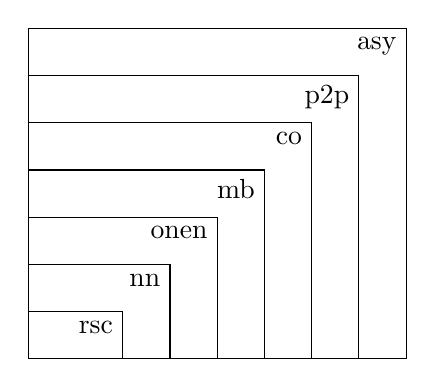
\begin{tikzpicture}[scale=0.6]
  % list of labels in order (from smallest to largest)
%   \def\labels{{rsc,nn,onen,mb,co,p2p,asy}}
  % loop to draw nested squares
  \foreach [count=\i] \lab in {rsc,nn,onen,mb,co,p2p,asy} {
    \draw (0,0) rectangle (\i+1,\i);
    \node[anchor=north east] at (\i+1,\i) {\lab};
  }
\end{tikzpicture}
\caption{Hierarchy of communication model semantics.}
\label{fig:coms}
\end{figure}

% TODO: dire che la proiezione non è monotona e che quindi non può essere
% passata ad altre semantica (ma altre sì tipo weak-k-synchronizability)

\begin{figure}[!ht]
    \centering
    \begin{tabular}{cc}
        \scalebox{0.6}{%
        \begin{msc}[draw frame=none, draw head=none, msc keyword=, 
                    head height=0px, label distance=0.5ex, 
                    foot height=0px, foot distance=0px]{}
            \declinst{p}{p}{}
            \declinst{q}{q}{}

            \mess[pos=0.2]{$m_1$}{p}{q}[2]
            \nextlevel
            \mess[pos=0.8]{$m_2$}{p}{q}
        \end{msc}%
        } &
        \scalebox{0.5}{%
        \begin{msc}[draw frame=none, draw head=none, msc keyword=, 
                    head height=0px, label distance=0.5ex, 
                    foot height=0px, foot distance=0px]{}
            \declinst{p}{p}{}
            \declinst{q}{q}{}
            \declinst{r}{r}{}

            \mess[pos=0.15]{$m_1$}{p}{r}[3]
            \nextlevel
            \mess[pos=0.8]{$m_2$}{p}{q}
            \nextlevel
            \mess[pos=0.8]{$m_3$}{q}{r}
        \end{msc}%
        } \\
        (a) asynchronous (\verb|asy|) & (b) peer-to-peer (\verb|p2p|) \\
        \scalebox{0.5}{%
        \begin{msc}[draw frame=none, draw head=none, msc keyword=, 
                    head height=0px, label distance=0.5ex, 
                    foot height=0px, foot distance=0px]{}
            \declinst{p}{p}{}
            \declinst{q}{q}{}
            \declinst{r}{r}{}
            \declinst{s}{s}{}

            \mess[pos=0.1]{$m_4$}{p}{s}[4]
            \nextlevel
            \mess[pos=0.8]{$m_1$}{p}{q}
            \nextlevel
            \mess[pos=0.2]{$m_2$}{r}{q}
            \nextlevel
            \mess[pos=0.8]{$m_3$}{r}{s}
        \end{msc}%
        } &
        \scalebox{0.6}{%
        \begin{msc}[draw frame=none, draw head=none, msc keyword=, 
                    head height=0px, label distance=0.5ex, 
                    foot height=0px, foot distance=0px]{}
            \declinst{p}{p}{}
            \declinst{q}{q}{}
            \declinst{r}{r}{}

            \mess{$m_1$}{p}{q}
            \nextlevel
            \mess{$m_2$}{q}{r}
        \end{msc}%
        } \\
        (c) mailbox (\verb|mb|) & (d) synchronous (\verb|synch|)
    \end{tabular}
    \caption{MSCs' Examples for various communication models.}
    \label{fig:msc_examples}
\end{figure}

\paragraph{Fully asynchronous}

In the fully asynchronous communication model (\verb|asy|), messages can be 
received at any time after they have been sent, and send events are 
non-blocking. This model can be viewed as an unordered ``bag'' in which 
all messages are stored and retrieved by processes when needed. It is also 
referred to as \emph{non-FIFO}. The formal definition coincides with that of 
an MSC. Figure~\ref{fig:msc_examples}.a illustrates an example of asynchronous 
communication.

\paragraph{Peer-to-peer} 
In the peer-to-peer (\verb|p2p|) communication model, any two messages sent from one 
process to another are always received in the same order as they are sent.
Alternative names are FIFO. An example is shown in Figure~\ref{fig:msc_examples}.b.

% A p2p-MSC is an MSC $M = (E,\to, \lhd, \lambda)$ where, for any two send events $s$ 
% and $s'$ such that $\lambda(s) \in \text{send}(p, q, \_), \lambda(s') in \text{send}(p, q, \_)$, 
% and $s \to^+ s'$, one of the following holds:
% - either $s, s' \in \text{matched}(M)$ with $s \lhd r$ and $s' \lhd r'$ and 
% $r \to^+ r'$,
% - or $s' \in \text{unmatched}(M)$.
% Note that we cannot have two messages $m 1$ and $m 2$, both sent by $p$ to $q$, 
% in that order, such that $m 1$ is unmatched and $m 2$ is matched; unmatched 
% message $m 1$ excludes the reception of any later message.

\paragraph{Causally ordered}
In the causally ordered (\verb|co|) communication model, messages are delivered 
to a process in accordance with the causal dependencies of their emissions. 
In other words, if there are two messages $m_1$ and $m_2$ with the same recipient, 
such that there exists a causal path from $m_1$ to $m_2$, then $m_1$ must be received 
before $m_2$. This notion of causal ordering was first introduced by Lamport under the 
name ``happened-before'' relation. In Figure~\ref{fig:msc_examples}.b, this 
causality is violated: $m_1$ should be received before $m_3$. Causal delivery 
is commonly implemented using Lamport's logical clock algorithm \cite{lamport2019time}.

% An MSC $M = (E, \to, \lhd, \lambda)$ is causally ordered if, for any two send $s$ and 
% $s'$, such that $\lambda(s) \in \text{send}(\_, q, \_), \lambda(s') \in \text{send}(\_, q, \_)$, and 
% $s \leq_{\text{hb}} s'$:
% - either $s, s' \in \text{matched}(M)$ and $r \to^* r'$, with $r$ and $r'$ receive 
% events such that $s \lhd r$ and $s' \lhd r'$.
% - or $s' \in \text{unmatched}(M)$.

% Note that in a \verb|co|-MSC we cannot have two send events $s$ and $s'$ addressed 
% to the same process, such that $s$ is unmatched, $s'$ is matched, and 
% $s \leq_{\text{hb}} s'$.

\paragraph{Mailbox}
In this model, any two messages sent to the same process, regardless of the sender, 
must be received in the same order as they are sent. If a process receives $m_1$ 
before $m_2$, then $m_1$ must have been sent before $m_2$. \verb|mb| coordinates all 
the senders of a single receiver. This model is also called FIFO $n-1$.
In Figure~\ref{fig:msc_examples}.c, an example for this communication model is shown.

% An MSC $M = (E, \to, \lhd, \lambda)$ is a \verb|mb|-MSC if it has a linearization 
% $\rightsquigarrow$ where, for any two send events $s$ and $s'$, such 
% that $\lambda (s) \in \text{send}(\_,q,\_), \lambda (s') \in \text{send}(\_,q,\_)$, and 
% $s \rightsquigarrow s'$
% - either $s,s' \in \text{matched}(M)$ and $r \rightsquigarrow r'$, where 
% $s \lhd r$ and $s' \lhd r'$,
% - or $s' \in \text{unmatched}(M)$.

\paragraph{FIFO 1-n}
This model (\verb|onen|) is the dual of \verb|mb|, it coordinates a sender with all the 
receivers. Any two messages sent by a process must be received in the same 
order as they are sent. These two messages might be received by different 
processes and the two receive events might be concurrent.

% An MSC $M = (E, \to, \lhd, \lambda)$ is a \verb|onen|-MSC if it has a linearization 
% $\rightsquigarrow$ where, for any two send events $s$ and $s'$, such 
% that $\lambda (s) \in \text{send}(p,\_,\_), \lambda (s') \in \text{send}(p,\_,\_)$ and 
% $s \to^+ s'$ (which implies $s \rightsquigarrow s'$)
% - either $s,s' \in \text{matched}(M)$ and $r \rightsquigarrow r'$, with 
% $r$ and $r'$ receive events such that $s \lhd r$ and $s' \lhd r'$,
% - or $s' \in \text{unmatched}(M)$.

\paragraph{FIFO n-n}
In this model (\verb|nn|), messages are globally ordered and delivered according to 
their emission order. Any two messages must be received in the same order 
as they are sent. These two messages might be sent or receives by any process 
and the two send or receive events might be concurrent. The FIFO \verb|n-n| 
coordinates all the senders with all the receivers.

% An MSC $M = (E, \to, \lhd, \lambda)$ is a \verb|nn|-MSC if it has a linearization 
% $\rightsquigarrow$ where, for any two send events $s$ and $s'$, such 
% that $s \rightsquigarrow s'$
% - either $s, s' \in \text{matched}(M)$ and $r \rightsquigarrow r'$, with $r$ 
% and $r'$ receive events such that $s \lhd r$ and $s' \lhd r'$,
% - or $s' \in \text{unmatched}(M)$.

\paragraph{Synchronous}
The synchronous (\verb|synch|) communication model imposes 
the existence of a scheduling such that any send event is 
immediately followed by its corresponding receive event. 
An example for this communication model is shown in Figure~\ref{fig:msc_examples}.d.
A formal definition is given later for this semantic (Definition~\ref{def:synch}).

\subsection{Multiparty Session Types}
Multiparty Session Types (MPST)~\cite{honda2008multiparty} 
provide a type-theoretic framework to specify and verify communication 
protocols among multiple participants. They ensure that communication 
follows a predefined structure, preventing errors such as deadlocks, 
orphan messages, and unspecified receptions. The 
\textbf{global specification} describes the overall communication 
protocol. From this, one derives the \textbf{local behaviors} of each 
participant via a \emph{projection} operation. The system's 
\textbf{processes} form the \emph{implementation}, defining how 
participants interact. With the definition of a \emph{typing system} 
and suitable \emph{type-checking rules}, one ensures that the 
implementation conforms to the local specification, thereby 
guaranteeing properties such as \emph{well-formedness}.  

% In this setting, the analogue of realizability is often called 
% \emph{session fidelity}: a property ensuring that the combined local 
% types behave exactly according to the global type. When the global 
% type satisfies syntactic restrictions, its projection is guaranteed 
% to be both realizable and deadlock-free, which corresponds to safe 
% realizability in the MSC setting.  

\subsubsection{Projectability}
A central notion in MPST is \emph{projectability}, which asks whether 
a global type can be faithfully projected into local specifications for 
each participant. If projection succeeds, the resulting local types 
interact without mismatches or unintended behaviors, effectively 
bridging global specifications and distributed implementations~\cite{honda2008multiparty}.  
Projectability is, therefore, comparable to the implementability
problem as have the same aim.
Projection algorithms, however, often reject natural protocols that 
fail to meet restrictive syntactic conditions. This difference between 
expressivity and safety has motivated extensions of the theory, with 
\cite{castagna2012global} being the only algorithm aiming for full 
completeness.

\subsubsection{Mixed and Sender driven choice}
A key restriction appears in branching. In the original framework \cite{honda2008multiparty,carbone2012structured}, 
choice is \textbf{sender-driven}: the first sender dictates the branch, 
ensuring safety but excluding many common patterns where multiple 
participants influence the decision~\cite{carbone2012structured}.  
Allowing \textbf{mixed choice} increases expressivity by permitting 
several initiators, but it also makes the implementability problem 
undecidable in general~\cite{barbanera2020choreography}.  

\subsection{Choreographies}
%todo


\subsection{Reduction to synchronous semantic}
The main idea of this work is that reasoning about implementability 
becomes more tractable under \emph{synchronous} 
semantics for automata-based solutions to the implementability problem. 
In synchronous communication, send and receive actions 
are tightly coupled, effectively removing nondeterminism 
caused by asynchronous message buffering. Several results exploit this 
observation by reducing the implementability problem under richer 
communication models (e.g.\ asynchronous or peer-to-peer FIFO) to the 
simpler synchronous case~\cite{alur2005realizability,di2023partial}.

Formally, one can show that if a global type is implementable in 
synchronous semantics, then under certain conditions it is also 
implementable in more general models such as peer-to-peer or mailbox 
semantics. This reduction requires constraints such as 
\emph{orphan-freedom} (no message is left unmatched) and
\emph{deadlock-freedom}.
The following theorem, currently a work in progress by my supervisors \cite{di2025realisability}, 
provides a characterization of a connection between 
peer-to-peer semantics and synchronous semantics:

\begin{theorem}
	A global type $G$ is implementable in \verb|p2p| iff:
	\begin{enumerate}
		\item $L_{\text{p2p}}(proj(G))$ is a set of sync MSCs;
		\item $proj(G)$ is orphan-free in p2p;
		\item $L_{\text{p2p}}(proj(G))$ is deadlock-free;
		\item $G$ is implementable in sync.
	\end{enumerate}
\end{theorem}

This result highlights the central role of synchronous semantics as a 
\emph{core model}: implementability in peer-to-peer systems 
can be reduced to the synchronous case provided the additional safety 
conditions are met. My own contribution focuses on the last item of the 
theorem, namely the problem of checking whether a given global type is 
implementable in synchronous semantics. This question is at the heart 
of the undecidability results presented in Section~\ref{sec:proof}, 
and motivates the need for the identification of new subclasses that 
enable new verification techniques along with tool support.